\textit{Le but de ce TP est d'implémenter deux algorithmes de résolution du problème de flot maximum : l'algorithme d'Edmonds-Karp et l'algorithme de Dinic. Nous commencerons par spécifier les fonctionnalités que devra implémenter notre programme, puis nous détaillerons la manière dont ces fonctionnalités ont été développées. Une troisième partie sera consacrée aux tests effectués sur les deux algorithmes ainsi qu'à l'analyse des résultats.}

\section{Spécifications fonctionnelles}

\subsection{Résolution du problème de flot maximum}

Le programme doit être capable de :
\begin{itemize}
\item générer et d'actualiser les graphes d'écarts successifs
\item calculer la valeur du flot obtenu à partir du graphe d'écart final
\item résoudre le problème de flot maximum en suivant l'algorithme d'\textbf{Edmonds-Karp}
\item résoudre le problème de flot maximum en suivant l'algorithme de \textbf{Dinic}
\item retourner la solution de manière exploitable pour l'analyse
\end{itemize}

Il faudra veiller à conserver la complexité des deux algorithmes, notamment en prenant garde aux structures de données et librairies utilisées.

\subsection{Génération aléatoire d'un réseau de transport}

La génération aléatoire de graphes de type réseau de transport permettra de tester les deux algorithmes. Il faudra veiller à ce que le graphe respecte les conditions d'un réseau de transport notamment la possession d'une source et d'un puits, la pondération des arcs (capacités), et assurer la connexité du graphe. La génération de ce réseau de transport devra être paramétrable selon la taille (nombre de sommets) et la densité (nombre d'arcs).

\section{Spécifications techniques}

\subsection{Programmation C++}
En plus de sa notoriété, nous avons choisi de développer l'application en C++ car il s'agit d'un bon compromis entre langage orienté objet et langage de bas niveau. Nous pourrons ainsi abstraire la gestion des graphes (notamment des structures de données) dans nos algorithmes, tout en gardant la possibilité d'optimiser le code grâce à la flexibilité du langage C.

\subsection{Structures de données}

\subsubsection{Graphes}
Les graphes peuvent êtres stockés à l'aide différents types de structures de données. Nous avons choisi d'en implémenter deux :  par listes d'adjacences et par matrice d'adjacences.
\begin{description}
\item[Listes d'adjacences] : chaque sommet possède la liste de ses voisins. Ces listes ont l'avantage d'allouer de la mémoire uniquement lorsqu'une information doit être stockée. 
\item[Matrice d'adjacences] : la mémoire allouée pour cette structure de données ne dépend que du nombre de sommets ($n^2$). Cette structure a l'avantage d'offrir un accès direct à un arc pour deux sommets donnés.
\end{description}

Dans un but d'optimisation mémoire, on utilise en général des listes d'adjacences lorsque l'on travail sur des graphes peu denses. En effet, la taille allouée par cette structure de données étant directement dépendante du nombre d'arcs, elle est donc réduite par rapport aux matrices d'adjacences. Sur des graphes très dense, on utilisera en revanche des matrices d'adjacences, permettant un accès aux données plus rapide. 

Les ressources matériels disponibles peuvent également orienter ce choix.

\subsection{Modélisation}
Afin de s'abstraire de la structure de donnée, nous avons choisi de créer une classe abstraite \texttt{AbstractGraph} dont deux classes fille héritent. Un graphe peut donc être de type \texttt{AdjacencyListGraph} ou \texttt{MatrixGraph}. Cela permet une grande généricité des algorithme développés, ce qui permet d'utiliser une structure de données de manière totalement détachée des algorithmes.
\begin{figure}[t]
\begin{center}
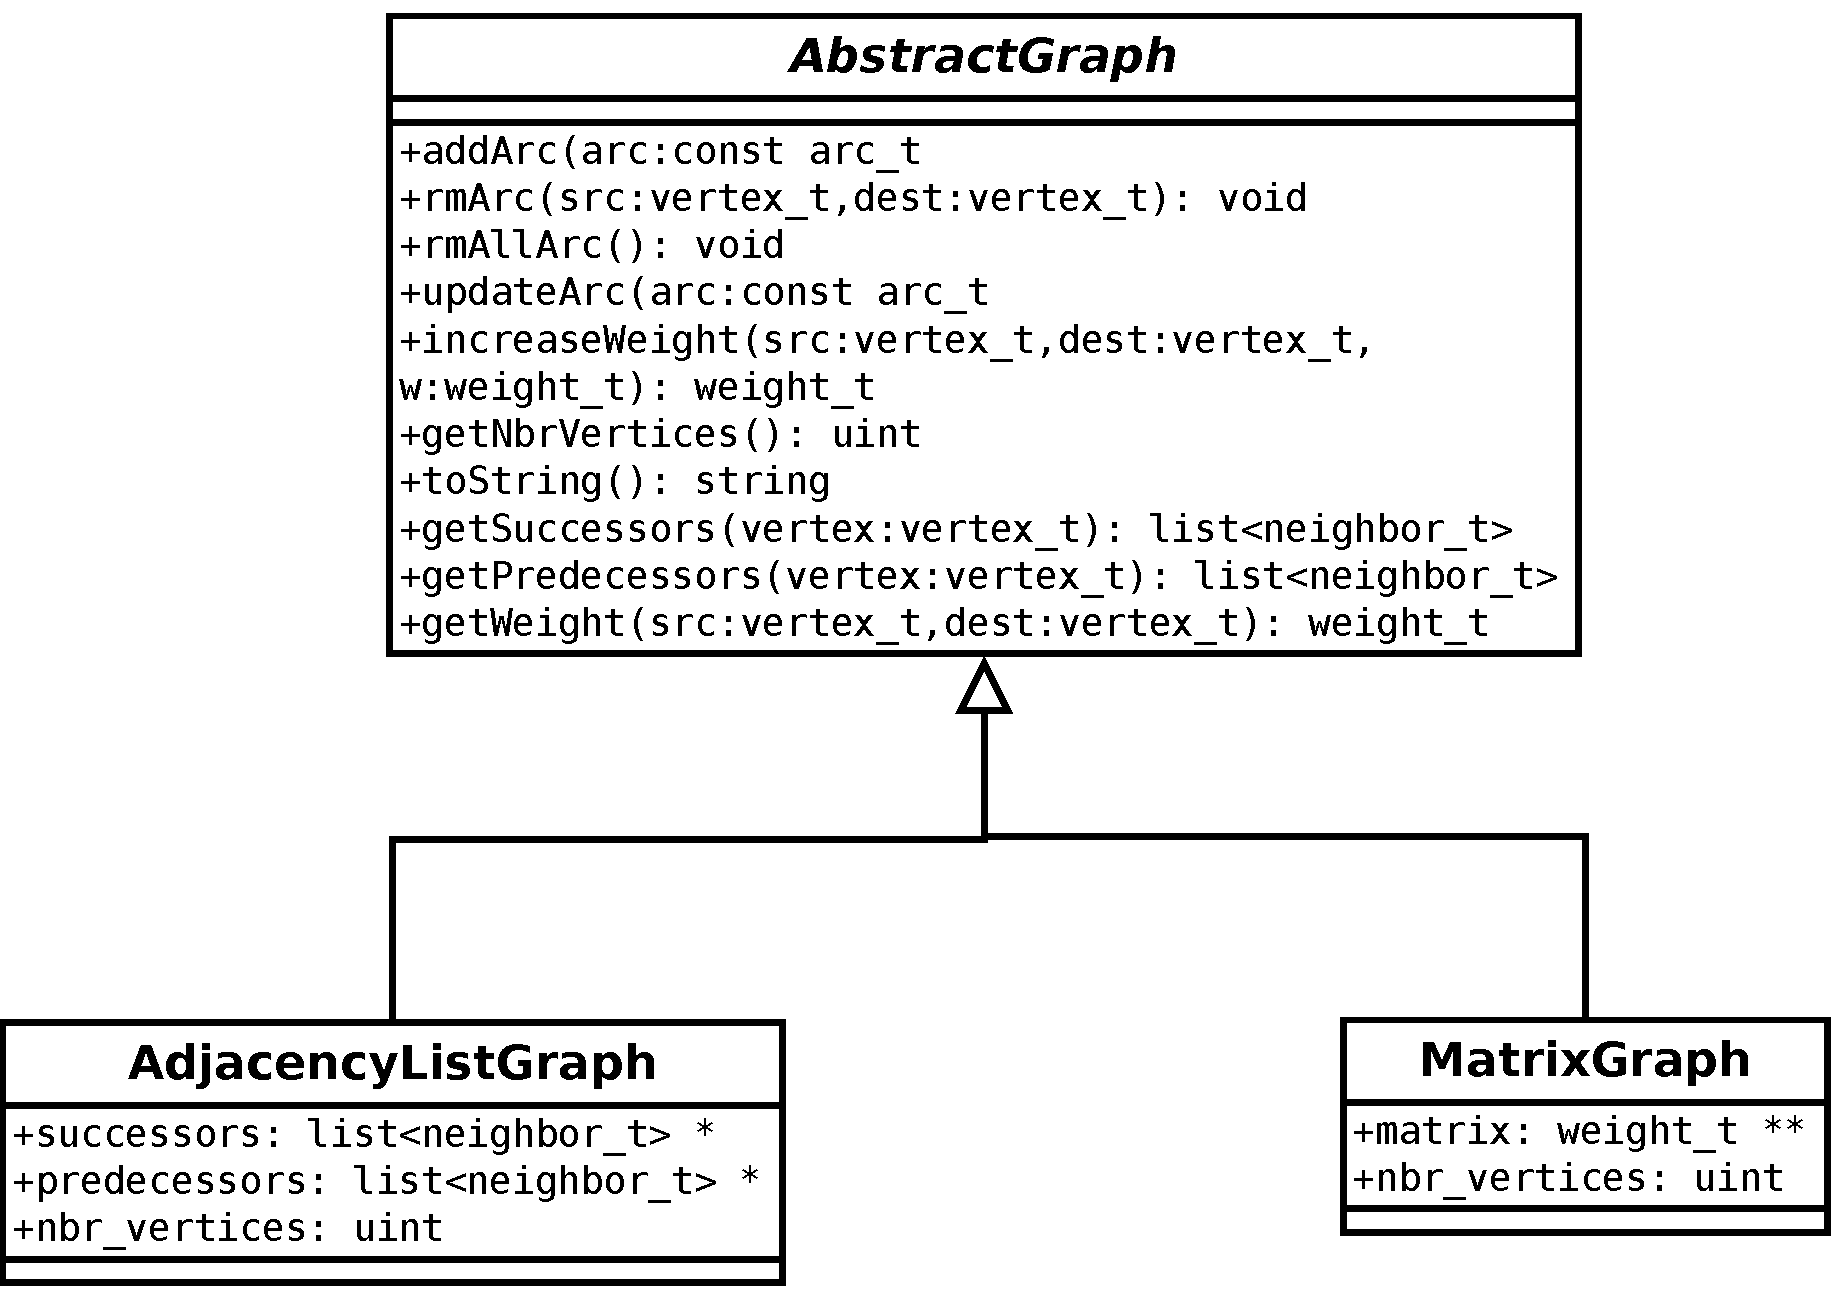
\includegraphics[width=\textwidth]{files/diag_class}
\end{center}
\caption{Diagramme de classes.}
\end{figure}

\FloatBarrier

\subsection{Types et structures}

Déclaration des types \texttt{weight\_t}, \texttt{vertex\_t} et \texttt{path\_t}, et des structures \texttt{edge}, \texttt{neighbor\_t}

\lstinputlisting[language=C++,morekeywords={}]{./sources/structs}

\subsection{Classe \texttt{AbstractGraph}}

Cette classe permet une abstraction des différentes représentations d'un graphe (structures de données utilisées). Elle déclare les méthodes qui doivent êtres implémentés dans les classes filles.

Header de la classe \texttt{AbstractGraph}

\lstinputlisting[language=C++,morekeywords={}]{./sources/AbstractGraph}

\subsubsection{Classe \texttt{AdjacencyListGraph}}
Cette classe représente un réseau de transport sous la forme
de deux listes d'adjacences : une représente les 
successeurs d'un sommet, l'autre les prédécesseurs.

Ce doublon d'information permet d'accélérer l'accès aux voisins d'un sommet, notamment à ces prédécesseurs. En effet, cette méthode nous permet d'accéder à une liste des prédécesseurs directement (complexité de $O(1)$) alors que l'accès via les listes des successeurs implique le parcours de toutes ces listes (complexité de $O(nm)$).

Ces doubles listes d'adjacences nous assurent un gain de performances en terme de rapidité, qui se fait au détriment de la quantité de mémoire utilisé, qui se trouve doublée.

Header de la classe \texttt{AdjacencyListGraph}

\lstinputlisting[language=C++,morekeywords={}]{./sources/AdjacencyListGraph}


\subsubsection{Classe \texttt{MatrixGraph}}

Header de la classe \texttt{MatrixGraph}

\lstinputlisting[language=C++,morekeywords={}]{./sources/MatrixGraph}

\subsection{Génération de réseaux de transport aléatoires}

\lstinputlisting[language=C++,morekeywords={}]{./sources/aleatoire}

\subsection{Procédures principales}

 \subsection{Algorithme de Dinic}
\subsubsection{Mise à jour du graphe d'écart}
\lstinputlisting[language=C++,morekeywords={}]{./sources/ecart}

\subsubsection{Calcul du flot bloquant}
\lstinputlisting[language=C++,morekeywords={}]{./sources/bloquant}

\subsubsection{Exécution de Dinic}
\lstinputlisting[language=C++,morekeywords={}]{./sources/dinic}

\section{Implémentation}

\subsection{Génération aléatoire de réseaux de transports}


\subsection{Edmonds-karp}

\subsection{Dinic}


\section{Tests \& résultats}

\subsection{Méthode de test}

\subsubsection{Série de tests}
Pour tester les performances des deux algorithmes implémentés, nous avons générer une série de problèmes à résoudre sur des réseaux de transports ayant les paramètres suivants :
\begin{itemize}
\item nombre de sommets variant de 100 à 1000 par palier de 100,
\item densité du graphe variant de 10\% à 100\% par palier de 10.
\end{itemize}
Pour chaque test (un nombre de sommets et une densité donnés), nous avons généré dix graphes afin de travailler sur des moyennes lors de l'analyse.

\subsubsection{GNU gprof}
Nous avons évalué les algorithmes en fonction de leurs temps d'exécution. Le temps réel d'exécution (real time) ayant peu de sens pour effectuer des statistiques correctes, nous avons choisi de mesurer les temps CPU (CPU time). Le temps CPU est le temps alloué au processus par le système d'exploitation sur le processeur. Contrairement au temps réel, le temps CPU est indépendant des autres processus en cours d'activité et aux interruptions systèmes : il s'agit du temps effectivement passé par le CPU pour traiter le processus.

L'analyse des temps CPU a été faite à l'aide de l'outil GNU gprof. Son utilisation requière l'ajout de l'argument \texttt{-pg} lors la compilation. A l'exécution du programme, un fichier \texttt{gmon.out} est généré. La commande \texttt{gprof} permet ensuite de créer un fichier texte de statistiques. Pour chaque méthode, un grand nombre de données sont disponibles, nous nous sommes intéressés principalement aux suivantes :
\begin{itemize}
\item pourcentage du temps CPU total,
\item temps CPU total,
\item temps CPU par appel, de manière cumulative (en prenant en compte les appel à d'autres fonctions) ou non.
\end{itemize}

\subsection{Analyse des résultats}